\documentclass[12pt,a4paper,oneside]{scrbook}
\usepackage{mystyle}

% faster tikz. Needs to be here because of overleaf
\usepgfplotslibrary{external}
\tikzexternalize[prefix=tikzexternalize/]

\makeatletter
\renewcommand{\todo}[2][]{\tikzexternaldisable\@todo[#1]{#2}\tikzexternalenable}
\makeatother


\date{\today}
% \publishers{Universität Stuttgart}

\begin{document}

\tikzexternaldisable
\begin{titlepage}
    \begin{tikzpicture}[overlay,remember picture,y=-1cm]
        % set a new origin [1]
        \coordinate (O) at (current page.north west);
        \draw[fill=white,draw=yellow] ($(O)+(6.51,9.32)$) rectanglenode[align=center]{
                \large Bachelorarbeit
                \\
                \\
                \Large \textbf{Anwendung von}\\
                \Large \textbf{Contraction Hierarchies und} \\
                \Large \textbf{Hierarchical Hub Labeling}\\
                \Large \textbf{auf Nicht-Straßengraphen}
                \\
                \\
                \large Christian Staib
            } ($(O)+(15.37,14.97)$);
    \end{tikzpicture}
\end{titlepage}
\tikzexternalenable

\clearpage

\chapter*{Kurzfassung}
Die Technik der Contraction Hierarchies (CH) und der Hierarchical Hub Labelings (HL) haben sich als äußerst wirksame Techniken zur Beschleunigung von Routenanfragen in Straßennetzwerken erwiesen. Die Anwendung auf Graphen außerhalb des Straßenverkehrs wurde weit weniger untersucht - ein Beispiel hierfür findet sich z.B. in [1] -, auch wenn in diesen Fällen ebenfalls eine schnellere Anfrage von Suchanfragen wünschenswert ist.

Ziel dieser Arbeit ist es, diese Fragestellung eingehender zu untersuchen. Es sind hierbei sowohl andere Graphtypen zu betrachten, als auch ggf. bessere Konstruktionsstrategien für CH bzw. HL zu entwerfen. Graphtypen, die potenziell von Interesse sind:

\begin{itemize}
  \item
    Sichtbarkeitsgraphen
  \item
    Gridgraphen, wie sie z.B. in Computerspielen vorkommen
  \item
    Kommunikationsgraphen
  \item
    Kollaborationsgraphen
  \item
    Linkgraphen (z.B. von Wikipedia)
\end{itemize}

\tableofcontents
\chapter{Einleitung}

\section{Problemstellung}
Sichtbarkeitsgraphen sind Graphen, die alle Knotenpaare miteinander verbinden, die sich \emph{sehen} können, auf deren Luftlinie sich also keine \emph{Hindernisse befinden}.
Aus einer Küstenlinie kann ein Sichtbarkeitsgraph erstellt werden, indem die Knoten mit allen Knoten verbunden werden, deren Luftlinie keine Küste kreuzt.
\autoref{fig:thessaloniki-visibility} zeigt einen Ausschnitt eines solchen Sichtbarkeitsgraphen.
Zu sehen ist der Hafen der griechischen Stadt Thessaloniki.
Dass der Ausschnitt einen Hafen zeigt, ist kein Zufall, solch ein Sichtbarkeitsgraph kann für das Finden von kürzesten Schiffsrouten benutzt werden.
\todo{Navigation in 2D ist fast immer Sichtbarkeitsgraph}

Das Finden von kürzesten Pfaden ist auf solchen Graphen deutlich rechenintensiver als etwa auf Straßengraphen mit vergleichbarer Knotenanzahl, da sie unter anderem einen hohen durchschnittlichen Knotengrad und keine inhärente Hierarchische Struktur besitzen.
Zwar gibt es Möglichkeiten den Graphen zu verändern und schneller Wege zwischen Knoten zu berechnen, etwa durch Triangulierung oder Rasterisierung, jedoch sind diese Wege nicht mehr garantiert optimal.

Im Folgenden wird untersucht, inwiefern sich zwei Techniken zum schnellen Finden von kürzesten Pfaden und kürzester Pfad Distanzen (\emph{Contraction Hierarchies} und \emph{Hierarchical Hub Labeling}), auf diese Graphen anwenden lassen.

\begin{figure}[ht]%
    \centering
    \subfloat[\centering aegaeis-visibility]{{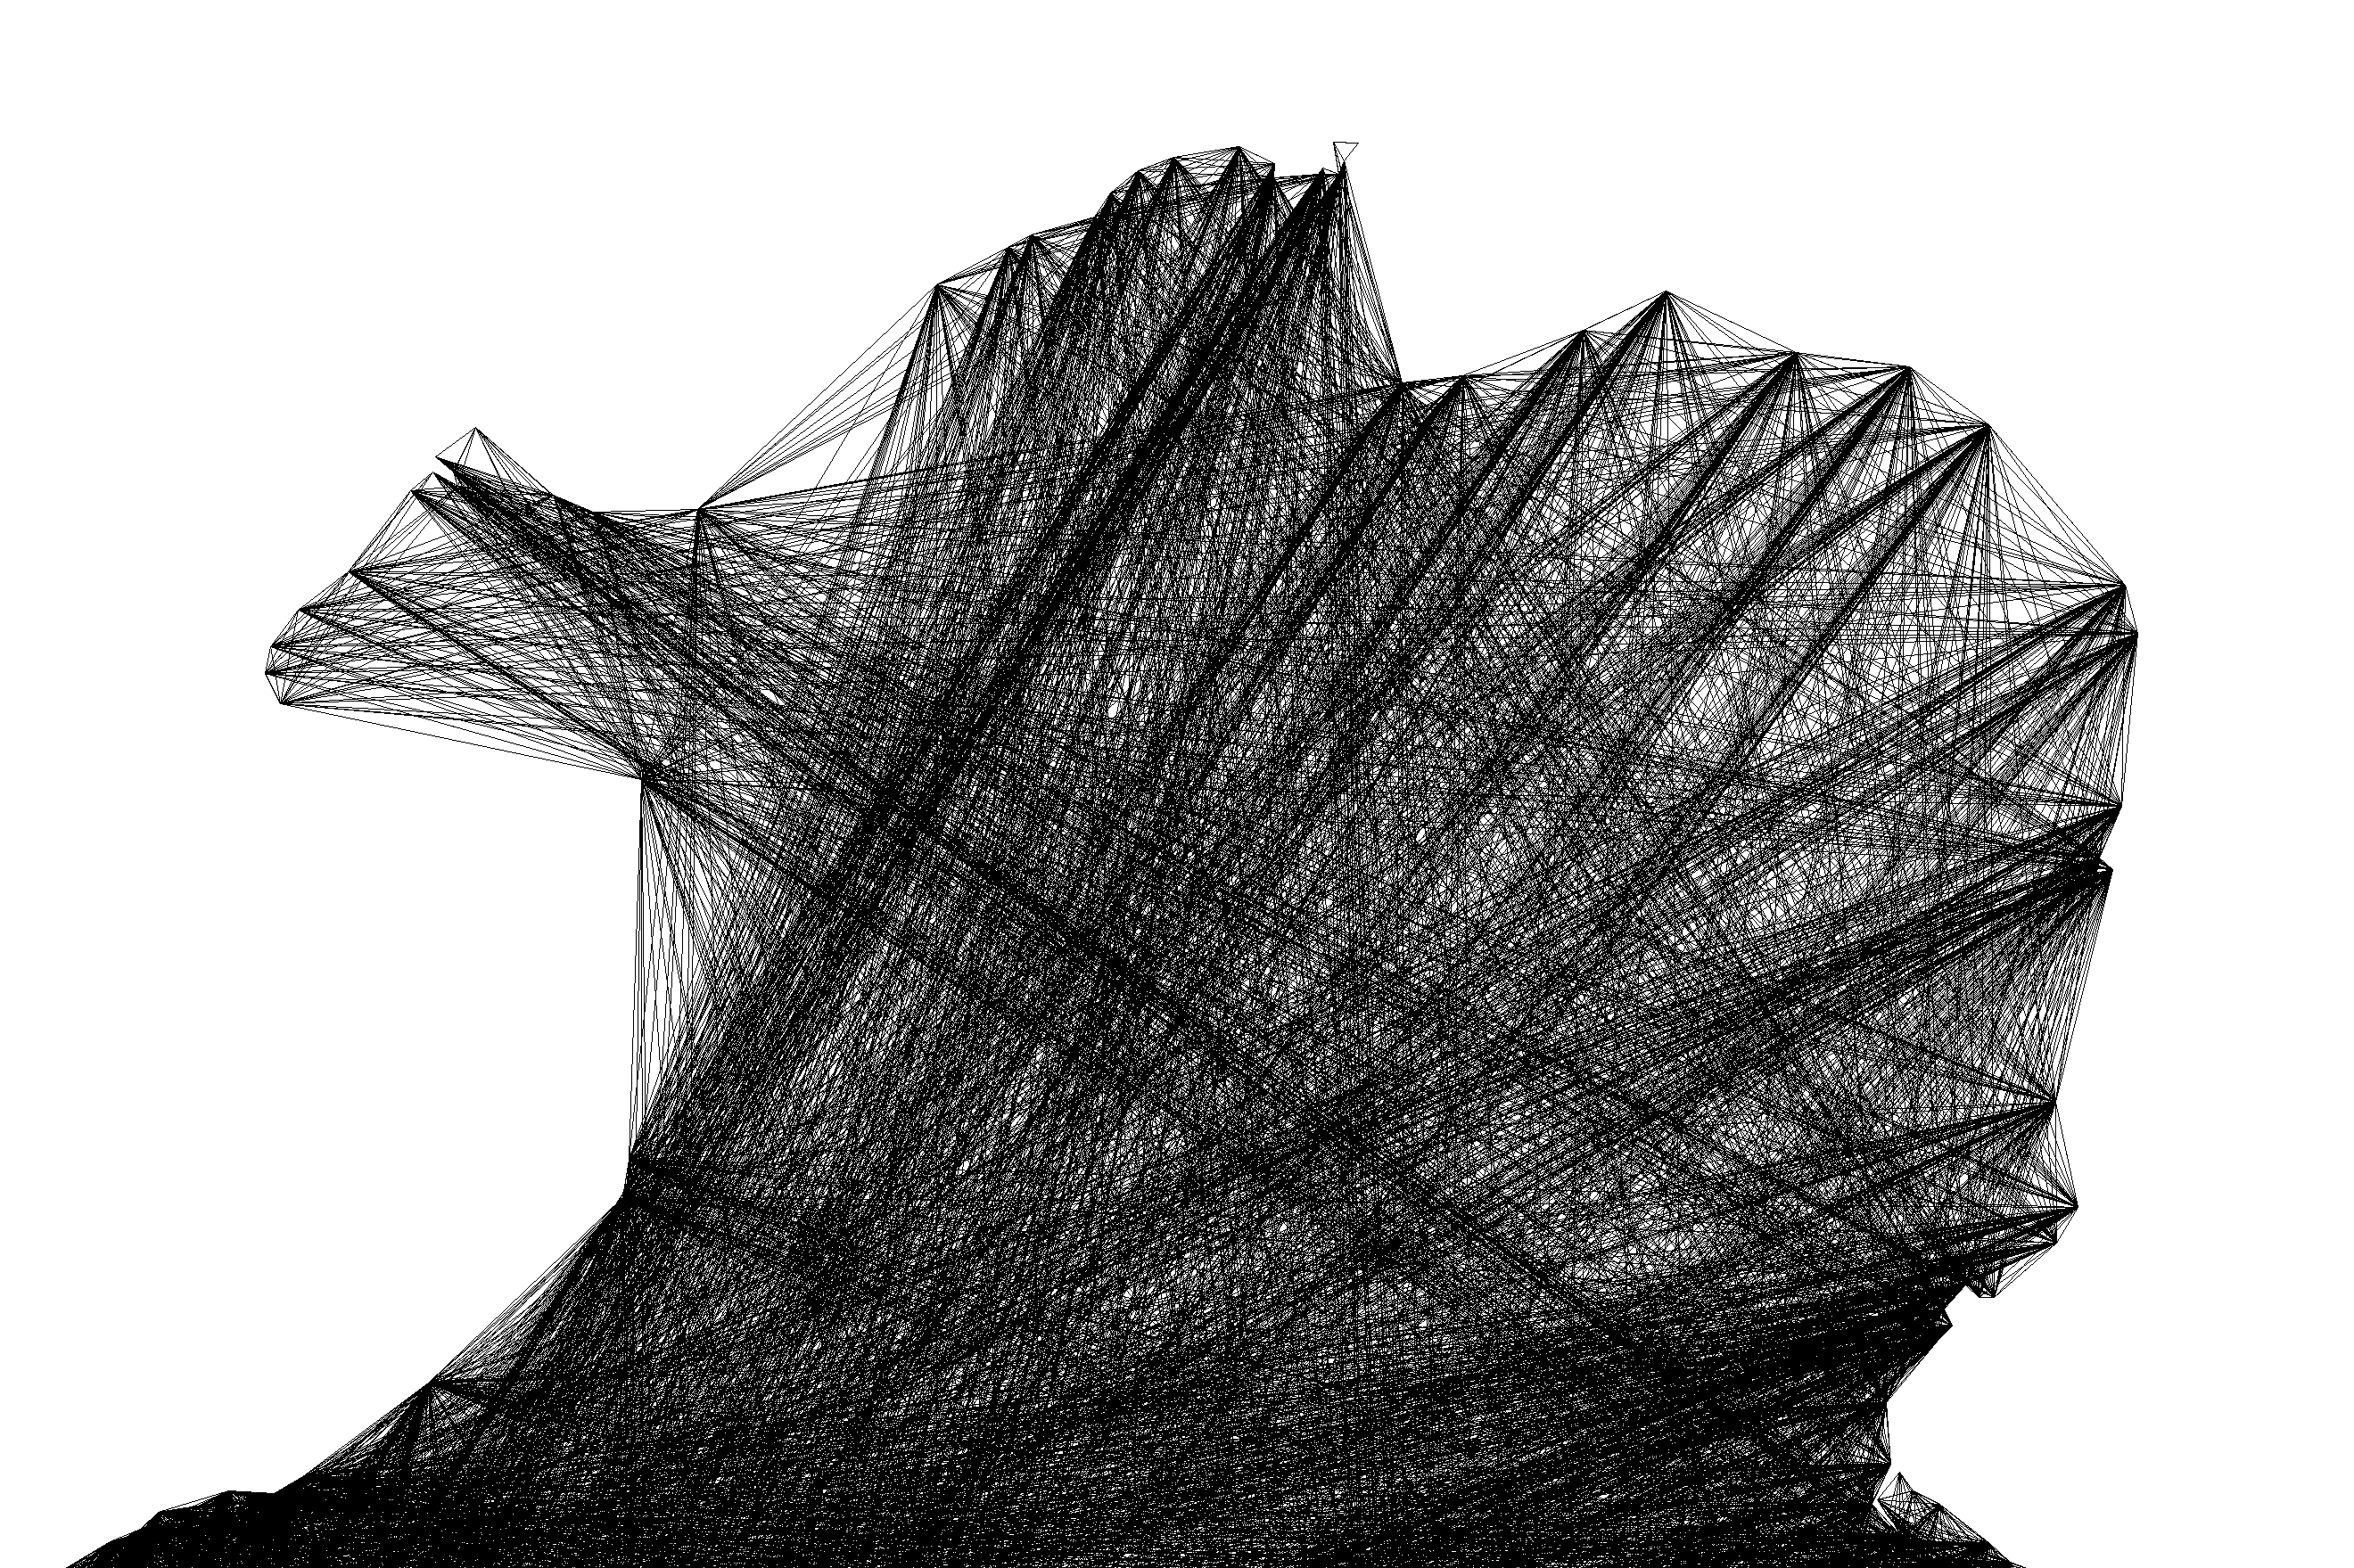
\includegraphics[width=.5\linewidth]{img/thessaloniki-visibility.png}}}%
    \caption{Sichtbarkeitsgraph des Hafens von Thessaloniki}%
    \label{fig:thessaloniki-visibility}%
\end{figure}

\section{Bearbeite Graphen}

Der Fokus dieser Arbeit liegt auf drei Sichtbarketisgraphen, welche jeweils einen Ausschnitt des Globus beinhalten.
Für jeden dieser 3 Graphen existiert zusätzlich eine Triangulation.
\autoref{table:input_graphs} listet die Graphen auf.
Die Graphen mit dem Präfix \emph{aegaeis} beinhalten das Ägäische Meer, mit \emph{medi} das Mittelmeer und mit \emph{pata} die Chilenische Fjorde.
Graphen mit dem Postfix \emph{visibility} sind Sichtbarkeitsgraphen, mit \emph{graph} Triangulationen.
Die bearbeiteten Graphen sind ungerichtet, werden im folgenden jedoch als gerichtet betrachtet.
Insbesondere ist die in \autoref{table:input_graphs} aufgelistete Anzahl an Kanten als gerichteter Graph zu interpretieren.
Die ungerichtete Kante $\{a, b\}$ wird also doppelt gezählt als $(a, b)$ und $(b, a)$.

\begin{table}[ht]
    \centering
    \begin{tabular}{
            l % Graph
            S[table-format = 7.0] % Zeit
            S[table-format = 9.0] % Zeit
            S[table-format = 4.1] % Zeit
        }
        \toprule
        {Graph}            & {\# Knoten} & {\# Kanten} & {$\varnothing$ Grad} \\ \midrule
        aegaeis-graph      & 524881      & 2795322     & 5.32562999994        \\
        aegaeis-visibility & 201040      & 310231834   & 1543.13486868        \\
        medi-graph         & 795606      & 4223566     & 5.30861506826        \\
        medi-visibility    & 310114      & 730772544   & 2356.46421638        \\
        pata-graph         & 2240339     & 11632900    & 5.1924731034         \\
        pata-visibility    & 1002171     & 315653758   & 314.969958221        \\ \bottomrule
    \end{tabular}
    \caption{Bearbeite Graphen}
    \label{table:input_graphs}
\end{table}

\subsection{Triangulation}

\todo{Daniel nach Details fragen, wie die Triangulation zustande gekommen ist.}

Erst Triangulierung. Wenn Dreiecke sehr schmal sind, dann ersetzen durch Subdreiecke.

Die Knoten eines triangulierten Graphen $G_g$ bilden eine Obermenge zur Menge der Knoten des dazugehörigen Sichtbarkeitsgraphen $G_v$.
Die Triangulation darf den kürzesten Pfad Abstand zweier Knoten $a, b$ nicht verkleinern, darf sie aber vergrößern.


\begin{figure}[ht]%
    \centering
    \subfloat[\centering aegaeis-graph]{{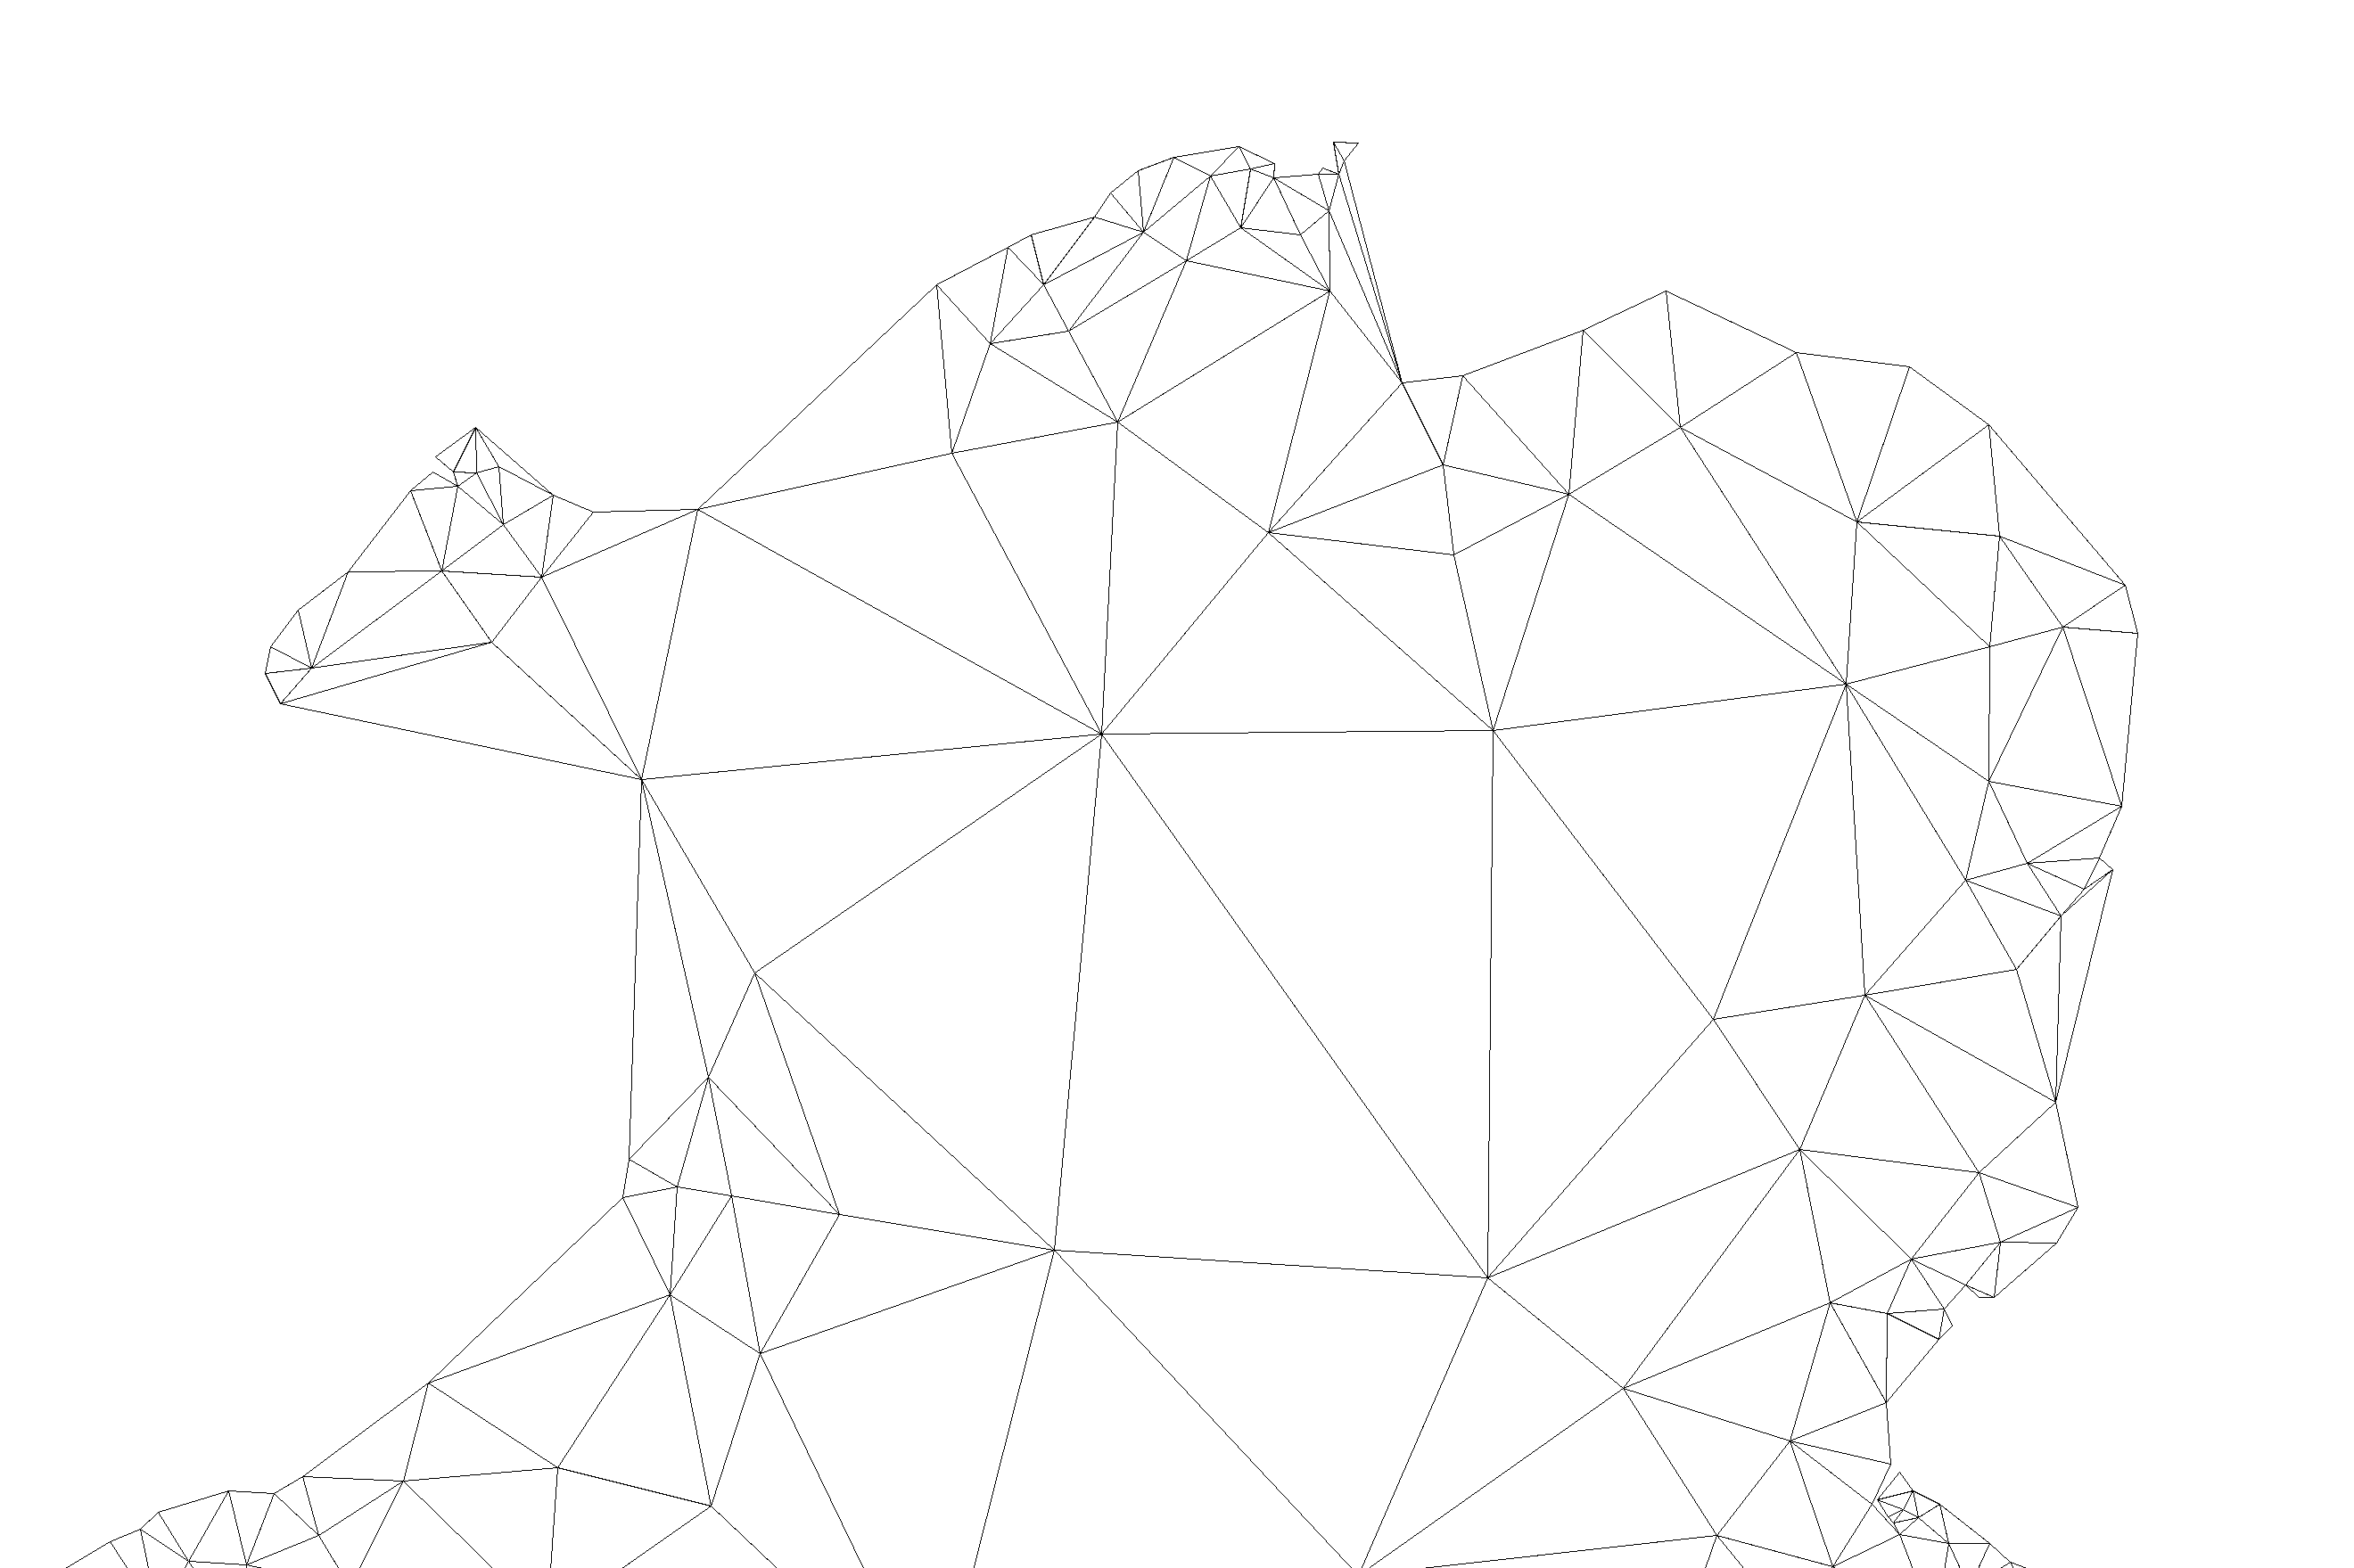
\includegraphics[width=.5\linewidth - 0.25cm]{img/thessaloniki-graph.png} }}%
    %\qquad
    \subfloat[\centering aegaeis-visibility]{{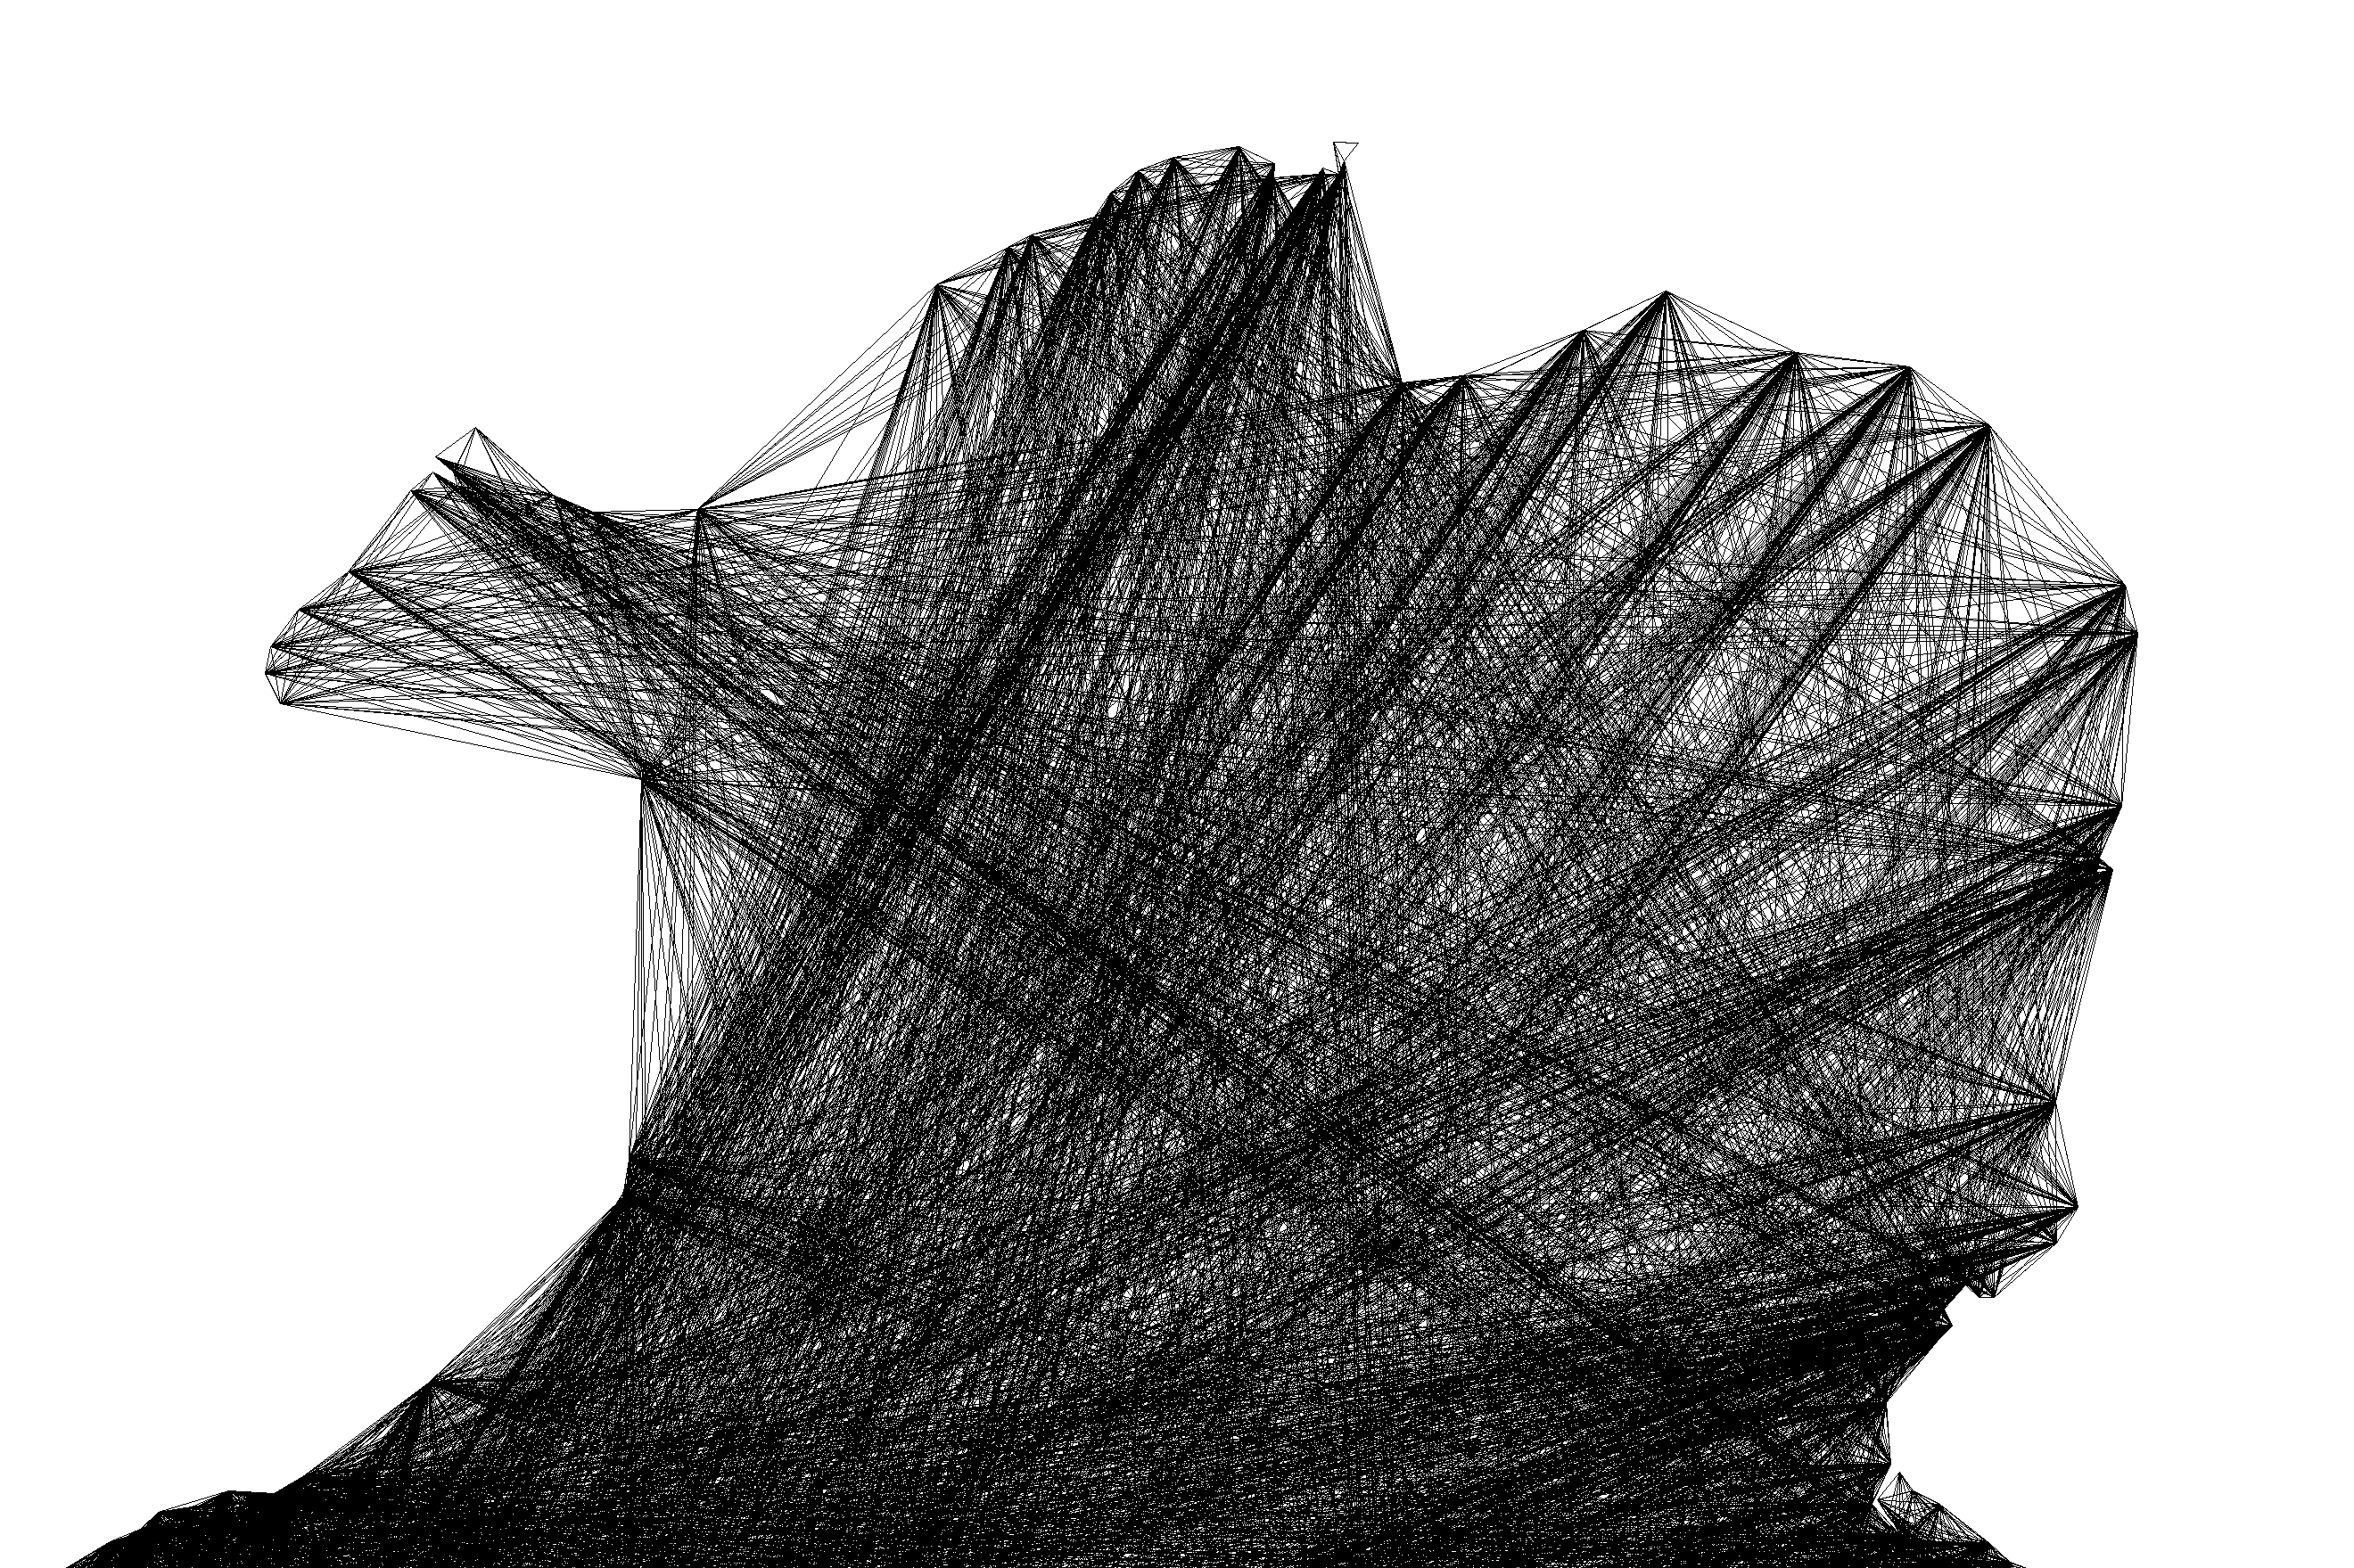
\includegraphics[width=.5\linewidth - 0.25cm]{img/thessaloniki-visibility.png} }}%
    \caption{Hafen von Thessaloniki}%
    \label{fig:thessaloniki}%
\end{figure}

\section{Speedup-Techniken}

Die betrachteten Speedup-Techniken zum Finden kürzester Pfade benötigen eine Phase der Vorbehandlung. (\emph{preprocessing}), damit danach kürzeste Pfad Anfragen (\emph{queries}) schneller beantwortet werden können.
Die für das Preprocessing benutzte Rechenzeit und der Memory-Overhead sollte dabei in einem sinnvollen Verhältnis zum Speedup und der Anzahl der Queries stehen.
Ist der Speedup besonders hoch, so lohnt es sich mehr in das Preprocessing zu investieren.


Beim Hierarchical Hub Labeling werden für jeden Knoten zwei \emph{Label} erstellt, welche den Suchbaum der Breitensuche repräsentieren.
Ein Vergleich beider Label liefert damit einen Knoten, welcher wieder auf dem kürzesten Pfad zwischen zwei Knoten liegt.
Eine genaue Beschreibung beider Techniken erfolgt in \autoref{chapter:ch} und \autoref{chapter:hl}.






\chapter{Graphen}

Ein Graph ist eine Struktur, die verwendet wird, um Beziehungen zwischen Objekten darzustellen.
Die Idee, Objekte durch Verbindungen zu verknüpfen, bildet die Grundlage für viele Anwendungen, unter anderem für die Routenplanung.
Graphen und (kürzeste) Pfade spielen aber auch jenseits davor eine wichtige Rolle, auf einem Wissengraph kann ein Pfad etwa dafür stehen, dass eine Aussage Wahr ist.
\autoref{graphs:fig:beispielgraph} zeigt einen Graphen, welcher im folgenden für Beispiele benutzt wird.

\begin{figure}[ht]
    \centering
    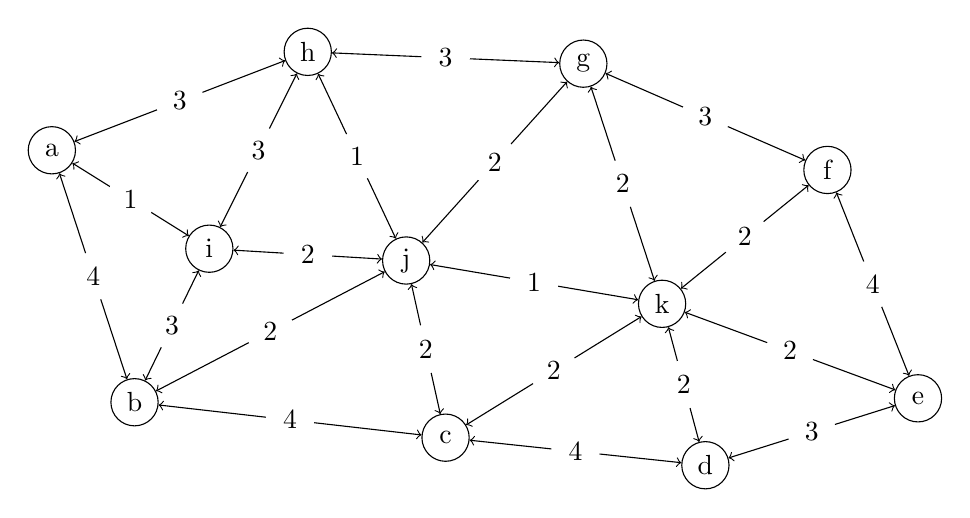
\begin{tikzpicture}
        % Nodes
        \node[circle, draw, minimum size=0.6cm, inner sep=0pt] at (0.5* 0.0, 0.5* 8.5)  (a)    {a};
        \node[circle, draw, minimum size=0.6cm, inner sep=0pt] at (0.5* 2.1, 0.5* 2.1)  (b)    {b};
        \node[circle, draw, minimum size=0.6cm, inner sep=0pt] at (0.5* 10.0, 0.5* 1.2)  (c)    {c};
        \node[circle, draw, minimum size=0.6cm, inner sep=0pt] at (0.5* 16.6, 0.5* 0.5)  (d)    {d};
        \node[circle, draw, minimum size=0.6cm, inner sep=0pt] at (0.5* 22.0, 0.5* 2.2)  (e)    {e};
        \node[circle, draw, minimum size=0.6cm, inner sep=0pt] at (0.5* 19.7, 0.5* 8.0)  (f)    {f};
        \node[circle, draw, minimum size=0.6cm, inner sep=0pt] at (0.5* 13.5, 0.5* 10.7)  (g)    {g};
        \node[circle, draw, minimum size=0.6cm, inner sep=0pt] at (0.5* 6.5, 0.5* 11.0)  (h)    {h};
        \node[circle, draw, minimum size=0.6cm, inner sep=0pt] at (0.5* 4.0, 0.5* 6.0)  (i)    {i};
        \node[circle, draw, minimum size=0.6cm, inner sep=0pt] at (0.5* 9.0, 0.5* 5.7)  (j)    {j};
        \node[circle, draw, minimum size=0.6cm, inner sep=0pt] at (0.5* 15.5, 0.5* 4.6)  (k)    {k};


        \draw[<->]  (a) edge node[circle, fill=white] {4} (b);
        \draw[<->]  (a) edge node[circle, fill=white] {3} (h);
        \draw[<->]  (a) edge node[circle, fill=white] {1} (i);

        \draw[<->]  (b) edge node[circle, fill=white] {4} (c);
        \draw[<->]  (b) edge node[circle, fill=white] {3} (i);
        \draw[<->]  (b) edge node[circle, fill=white] {2} (j);

        \draw[<->]  (c) edge node[circle, fill=white] {4} (d);
        \draw[<->]  (c) edge node[circle, fill=white] {2} (j);
        \draw[<->]  (c) edge node[circle, fill=white] {2} (k);

        \draw[<->]  (d) edge node[circle, fill=white] {3} (e);
        \draw[<->]  (d) edge node[circle, fill=white] {2} (k);

        \draw[<->]  (e) edge node[circle, fill=white] {4} (f);
        \draw[<->]  (e) edge node[circle, fill=white] {2} (k);

        \draw[<->]  (f) edge node[circle, fill=white] {3} (g);
        \draw[<->]  (f) edge node[circle, fill=white] {2} (k);

        \draw[<->]  (g) edge node[circle, fill=white] {3} (h);
        \draw[<->]  (g) edge node[circle, fill=white] {2} (j);
        \draw[<->]  (g) edge node[circle, fill=white] {2} (k);

        \draw[<->]  (h) edge node[circle, fill=white] {3} (i);
        \draw[<->]  (h) edge node[circle, fill=white] {1} (j);

        \draw[<->]  (i) edge node[circle, fill=white] {2} (j);

        \draw[<->]  (j) edge node[circle, fill=white] {1} (k);
    \end{tikzpicture}
    \caption{Beispielgraph}
    \label{graphs:fig:beispielgraph}
\end{figure}

\section{Definitionen}
Damit in den nachfolgenden Kapiteln sinnvoll argumentiert werden kann, ist es notwendig, einige Begriffe zu definieren.

\begin{definition}[Graph]
    Sofern nicht anders angegeben wird im folgenden Graph als eine Bezeichnung für einen endlichen, gerichteten Graph mit Kantengewichten, ohne Mehrfachkanten und Schleifen, verwendet.

    Als Schreibweise wird $G = (V, E)$ verwendet, wobei $V$ die Knotenmenge und $E$ die Kantenmenge ist. Eine Kante ist ein Tupel $(t, h, w)$. $t \in V$ wird als \emph{Fuß} (Tail), $h \in V$ als \emph{Kopf} (Head) und $w \in \mathbb{R}^+$ als \emph{Gewicht} (Weight) bezeichnet. Gelegentlich wird auch nur $(t, h)$ geschrieben, um auszudrücken, dass zwei Knoten verbunden sind. Da ein Graph keine Mehrfachkanten zulässt, verweiste diese Schreibweise auch eindeutig das Kantengewicht.

    Wird $G$ als ungerichtet bezeichnet, dann gilt $(t, h, w) \in E \Leftrightarrow (h, t, w) \in E$ und $(t, h)$ kann als $\{ t, h \}$ geschrieben werden.
\end{definition}

Das Gewicht der Kanten ist hierbei auf positive reelle Zahlen begrenzt, da das Verwenden eines Kantengewichtes $0$ dazu führen kann, dass ein kürzester Pfad mehrfach einen Teilpfad der Länge 0 durchläuft.
Negative Kantengewichte erschweren die Definition und Argumentation, sodass hier auf diese nicht weiter eingegangen wird,

\begin{definition}[Nachbar]
    Sei $G = (V, E)$. Ein Knoten $u \in V$ heißte \emph{Vorgänger} eines Knoten $v \in V$ wenn $(u, v) \in V$. $v$ ist in dann ein \emph{Nachfolger} von $u$.
    Ist $G$ ungerichtet, so spricht man beides mal von \emph{Nachbarn}.
\end{definition}

Die Anzahl der Nachbarn eines Knotens bezeichnet seien \emph{Grad}, wobei bei gerichteten Graphen vom \emph(Ein-) und \emph{Ausgangsgrad} gesprochen wird.
Hat ein Knoten keine Vorgänger oder Nachfolger, so nennt man ihn \emph{isoliert}.

\begin{definition}[Pfad]
    Ein Pfad $p$ auf einem Graph $G = (V, E)$ ist eine Folge von Knoten $(v_1, \dotsc, v_n)$, für die gilt, dass benachbarte Knoten im Pfad durch eine Kante in $G$ verbunden sind.
    Der Knoten $v_1$ wird Startknoten, $v_n$ Zielknoten genannt.
    Die Summe der Kantengewichte aller Kanten $(v_i, v_{i + 1})$ wird \emph{Länge}, die Anzahl der Kantennutzungen ($n - 1$) \emph{Hop-Länge} genannt.
\end{definition}

Häufig wird für den Startknoten der Buchstabe $s$ (Source) und für den Zielknoten $t$ für Target verwendet.
Zwischen zwei Knoten kann es Pfade unterschiedliche Länge geben, dies führt zur Definition des kürzesten Pfades.

\begin{definition}[Kürzester Pfad]
    Ein Pfad $p$ ist \emph{ein kürzester Pfad}, wenn die Länge von $p$ unter allen Pfaden von $v_1$ nach $v_n$ minimal ist.
    Die Länge des kürzesten Pfades wird als \emph{Abstand} von $v_1$ und $v_n$ bezeichnet.

    Die Funktion ${spd} \colon V \times V \to \mathbb{R}^+ \cup \{ \infty \} $ (shortest path distance) weist einem Knotenpaar den Abstand zu, wobei dieser unendlich ist, wenn kein Pfad zwischen ihnen existiert.
    Sei dann $P \subset V \times V$ die Menge der Knoten, zwischen denen ein Pfad existiert.
    Dann weist ${sp} \colon P \to V \times V \times \dots \times V$ (shortest path) einem Knotenpaar einen kürzesten Pfad zu.
\end{definition}

Zusätzlich zum Finden eines Pfades zwischen zwei Knoten ist es häufig notwendig die kürzesten Pfade von einem Knoten zu allen anderen Knoten zu finden.
Auch die Umkehrung dieses Problem ist Interessent, also die kürzesten Pfade von allen Knoten zu einem Knoten zu bestimmen.
Diese Probleme sind äquivalent, da das Finden aller kürzesten Pfade zu einem Knoten auf einem Graph $G$ dem Finden aller kürzester Pfade auf dem Umkehrgraph $G^T$ entspricht.

\begin{definition}[Umkehrgraph]
    Sei $G = (V, E)$ ein Graph. Dann ist $G^T = (V, E^T)$ mit $(t, h, w) \in E \Leftrightarrow (h, t, w) \in E^T$ der \emph{Umkehrgraph} von $G$.
\end{definition}

Ein ungerichteter Graph ist hier bei selbst ein Umkehrgraph.

\begin{definition}[Hitting-Set]
    Sei $G = (V, E)$ ein Graph und $P$ eine Menge an Pfaden auf $G$.
    Ein Hitting-Set $H = \subset V$ ist eine Menge an Knoten, so dass jeder Pfad $p \in P$ mindestens einen Knoten aus $H$ enthält
\end{definition}

Ein triviales Beispiel für ein Hitting-Set ist $V$ selbst, im Weiteren sind jedoch möglichst kleine Hitting-Sets nützlich.
Das Finden kleinst möglicher Hitting-Sets ist NP-vollständig \cite{Kar72}.
Der Greedy-Algorithmus \ref{graphs:alg:greedy-hitting-set} bietet jedoch eine Approximation in polynomieller Zeit an.

\begin{algorithm}
    \caption{Greedy Hitting-Set}
    \begin{algorithmic}[1]
        \Require Knotenmenge $V$, Pfade $P$ über $V$
        \Ensure Hitting-Set $H$

        \State $H \gets \emptyset$

        \State

        \While{$P \neq \emptyset$}
        \State Wähle $v \in V$ mit $\abs{ \{ p \mid p \in P \colon v \in p \}}$ maximal
        \State $H \gets H \cup \{  v \}]$
        \State $P \gets P \setminus \{p \in P \mid v \in p\}$
        \EndWhile

        \State

        \State \Return $H$
    \end{algorithmic}
    \label{graphs:alg:greedy-hitting-set}
\end{algorithm}


\section{Graphentypen}
\subsection{Straßengraphen}\label{graphs:strassengraphen}

Straßengraphen stellen eine spezielle Klasse von Graphen dar, die  Eigenschaften aufweisen, welche sie von allgemeinen Graphen abgrenzen.
Eine ihrer auffälligsten Merkmale ist, dass sie nahezu planar sind, sie also fast in der Ebene darstellen lassen, wobei Ausnahmen in Form von Über- und Unterführungen existieren.
Die Kantengewichte können etwa dem Luftlinienabstand oder der Reisezeit entsprechen, wobei sich letzter im Verlauf der Zeit ändern, etwa durch Stau oder Bauarbeiten.
Sie haben einen relativ geringen durchschnittlichen Knotengrad, Kreuzungen von mehr als zwei Straßen sind selten.

Sie besitzen sie eine hierarchische Struktur: Einfach gesagt, je schneller auf einer Straße gefahren werden darf, desto wichtiger is diese für das Finden von kürzesten Pfaden.
Die Wichtigkeit der benutzten Straßen eines kürzesten Pfades steigt im Allgemeinen an, bis etwa eine Autobahn erreicht wird, und nimmt schließlich wieder ab, bis das Ziel erreicht wird.

Eine weitere Eigenschaft dieser hierarchischen Struktur ist, dass hinreichend lange Pfade durch ein vergleichbar kleines Hitting Set getroffen werden.
Diese Knoten können etwa Autobahnkreuzen und Anschlussstellen sein.
Diese Beobachtung führt zur Definition der sogenannten Highway Dimension, einem Konzept, das von \cite{abraham2010highway} eingeführt wurde.

\subsection{Nicht-Straßen-Graphen}

Alle Graphen, die keine Straßengraphen sind, werden als Nicht-Straßen-Graph bezeichnet.
Da sie durch den Ausschluss der Straßengraphen definiert werden, haben sie keine gemeinsamen Eigenschaften, jedoch könne weite Teilklassen definiert werden.

\subsubsection{Sichtbarkeitsgraphen}

\todo{Funke. Was soll ich schreiben Stichwörter pls, Gummiband Eigenschaft}

\begin{definition}[Sichtbarkeitsgraph]
    Sei $V$ eine Menge an Punkten in einem euklidische Raum $A$. Sei $P$ eine Menge an Polygonen im selben Raum.

    Der Sichtbarkeitsgraph $G = (V, E)$ enthält alle Kanten $(t, h)$, die kein Polygon schneiden.
    Ihr Kantengewicht ist durch den euklidischen Abstand defniert.
\end{definition}



\subsubsection{Die Graphen im Detail}

\todo{Bilder}

\section{Dijkstra Algorithmus}

Die Angabe wie aufwändig die Suche eines kürzesten $(s, t)$ Pfades für einen Computer ist, lässt sich schwer in einer Metrik ausdrücken, denn die Zeit, welche für die Suche benötigt wird, ist von der verwendeten Hardware abhängig.
Ein Möglichkeit diese Aufwändigkeit zu beziffern, ist der \emph{Dijkstra Rank}.
Dieser gibt an, wieviele Knoten in einer Dijsktra-Suche von $s$ aus expandiert werden müssen, bis man von $t$ erreicht.

\todo{Ich habe gelesen, dass Dijkstra die meiste Zeit in Queue verbringt. Kann ich das wieder finden, oder selber perfen?}

Ebenfalls interesannt sind die Warteschlagen (Queue) Operationen, diese können auch Hinweise darauf geben, was genau die Suche in einem Graph so teuer macht.
Hierbei sind die \emph{Queue Pops} die Anzahl, wie oft Knoten aus der Warteschlange entommen wurde.
Wenn eine Warteschlange mit \emph{Decrease-Key} Funktion benutzt wird, unterscheidet sie sich nicht vom Dijsktra Rank.
Die \emph{Queue Pushs} geben an, wie oft Knoten aus der Warteschlange entommen werden.


\todo{Dijkstra Algorithmus erklären und Dijkstra Paper zitieren}
\begin{algorithm}[ht]
    \caption{Dijkstra Algorithmus}
    \begin{algorithmic}[1]
        \Require Graph $G = (V, E)$, Startknoten $s \in V$, Zielknoten $t \in V$
        \Ensure ${dist}$, ${pre}$
        \State // Initialisiere Distanz- und Vorgänger-Funktion
        \ForAll{$v \in V$}
        \State ${dist}(v) \leftarrow \infty$
        \State ${pre}(v) \leftarrow {none}$
        \EndFor


        \State
        \State // Initialisiere Vorrangwarteschlange
        \State ${dist}(s) \leftarrow 0$
        \State $Q\leftarrow \{ s \}$

        \State
        \While{$Q \neq \emptyset$}
        \State $u \leftarrow{extract\_min}(Q)$\label{graphs:dijkstra:pop}

        \State
        \State // Beende frühzeitig wenn Zielknoten gefunden wurde
        \If {$u = t$}
        \State \textbf{break}
        \EndIf

        \State
        \State // Aktualisiere Nachbarn
        \ForAll{$(u, v, w) \in E$}
        \If {${dist}(u) + w < {dist}(v)$}
        \State ${dist}(v) \leftarrow {dist}(u) + w$
        \State ${pre}(u) \leftarrow v$
        \State $Q = Q \cup \{ v \}$
        \EndIf
        \EndFor

        \EndWhile

        \State
        \State \Return ${dist}$, ${pre}$
    \end{algorithmic}
\end{algorithm}


\section{Dateiformat}

Die in dieser Arbeit verwendeten Graphen sind im \emph{.fmi} Dateiformat gespeichert, welches wie folgt definiert ist:

\begin{definition}[FMI Dateiformat]
    Eine Datei im .fmi Format besteht aus den folgenden Zeilen (in der angegebenen Reihenfolge):
    \begin{enumerate}
        \item
              Beliebig viele Kommentarzeilen, die mit einem \# beginnen.

        \item
              Eine leere Zeile.

        \item
              Eine Zeile, die die Anzahl der Knoten enthält.

        \item
              Eine Zeile, die die Anzahl der Kanten enthält.

        \item
              Knoten-Zeilen im Format: \texttt{KnotenId1 KnotenId2 Breitengrad Längengrad Höhe}

        \item
              Kanten-Zeilen im Format: \texttt{FußId1 KopfId2 Gewicht Typ Geschwindigkeit}

    \end{enumerate}
\end{definition}

Für die in dieser Arbeit verwendeten Graphen sind die Felder für Höhe, Typ und Geschwindigkeit nicht von Bedeutung, sie enthalten jeweils den Wert 0.

\section{Datenstrukturen}

Vertices sind natürliche Zahlen bzw uint32.
Ein Graph enthält idealerweise keine isolierten Knoten.
isolierte Knoten sind doof für dijkstra und co.
Die Menge der Knoten ist definiert durch Ihre Anzahl.
Gibt es $n \in \mathbb{N}$ Knoten, so sind es $0, \dotsc, n - 1$.
Ein Graph der diese Eigenschaft nicht erfüllt, kann durch eine Mapping der Knoten in die Form gebracht werden.

Jenachdem was mit dem Graph gemacht werden soll, sind verschiedene Eigenschaften von Vorteil.
Manchmal ist eine effiziente Nachbar Abfrage wichtig,
Manchmal das bearbeiten des Graphes, einfügen oder löschen von Knoten

Es wurde ein dyn Trait benutzt, welches eine Overhead hat und kein inlining zulässt.
Dafür lassen sich verschiedene Methoden vergleichen.

Die Grundlegenden Implementierungen kennen nur ihre Vorgänger.
Ein Reversibe Graph besteht aus einem Graph und seinem Umkehrgraph.
Gleiche Datenstruktur.

\subsection{VecVecGraph}
Ein Vec mit pro Knoten ein Vec.
Der innere Vec speichert Tuple aus (Vertex, Distanz).
Der innere Vec ist nach Vertex sortiert.

Ein Knoten kann so mit eine binären Suche gefunden werden.
Doch ab einem großen Grad wird diese Suche teuer.
Das einfügen und Löschen ist auch etwas teuere, da die übrigen Elemente geschoben werden müssen

Das finden von Nachbarn geht aber schnell, weil kein unbenutzer Platz dazwischen ist.

\subsection{VecHashMap}
Ein Vec mit pro Knoten eine HashMap
Die innere HashMap speichert Vertex -> Distanz.
So kann schnell ein Knoten gefunden werden.

Das finden von Nachbarn ist etwas langsamer, da unbenutzter Platz zwischen den Hash Einträgen.

Das einfügen und löschen ist günstig.

Vielleicht wäre IndexMap noch spannend.
Schnelles finden von Nachbarn.
Schnelles Iterieren.

Einfügen und löschen etwas teuerer.

\subsection{VecGraph}
Zwei Vecs.
Ein Index Vec mit pro Knoten ein Eintrag (u32, u32).
Dieser Eintrag gibt den Startindex und Stopindex des des zweiten Vecs an.
Dieser ist ein Vec (Vertex, Distanz).

Das bietet den Vorteil, dass man die Kanten zusätzlich sortieren kann, für besser Cache lokalität.
Kanten häufig benutzter Knoten können so an einem Ende des Vec grupiert werden.
\chapter{Contraction Hierarchies}\label{chapter:ch}

\todo{Historie und Zitieren}

Die follgende Definition versucht unabhängig einer ERstellung zu argumentieren.

\begin{definition}[Level]
    Sei $G = V, E$ ein Graph.
    Sei $L \subseteq \mathbb{N}$ mit $\abs{L} = \abs{V}$.
    Dann wird eine bijketive Funktion ${vtl} \coloneq V \to L$ \emph{vertex-to-level} Funktion genannt.
    Ihre Umkehrfunktion ${ltv}$ wird \emph{level-to-vertex} Funktion genannt.
\end{definition}

\begin{definition}[Upward Graph]
    Sei $G = (V, E)$ und ${vtl}$ eine \emph{vertex-to-level} Funktion dazu. Dann ist $G_u = (V, E_u)$ ein \emph{upward Graph} zu $G$ wenn gilt:
    \begin{enumerate}
        \item\label{ch:definition:legal_edges}
        $E_u$ enthält nur Kanten $(t, h, w)$ mit $t, h \in V$ und $w \in \mathbb{N}$ für die ${vtl}(t) < {vtl}(h)$ und $w >= {spd}_{G}((t, h))$ gilt.

        \item\label{ch:definition:upward}
        $E_u$ enthält mindestens alle Kanten $(t, h, {spd}_{G}((t, h)))$ mit $t, h \in V$, für die gilt, dass $h$ das größte und $t$ das zweitgrößte Level auf allen kürzesten Wege auf $G$ von $t$ nach $h$ hat.
    \end{enumerate}
\end{definition}

Der Name des upward Graphen ergibt sich daher, dass die Suche in einem upward Graph auf das Level bezogen nur \emph{aufwärts} geht.

Betrachten wir das ganze an dem bereits definierten Beispielgraph.
Sei ${vtl}$ definiert durch die Abbildung
$\bigl(\begin{smallmatrix}
            a & b & c & d & e & f & g & h & i & j & k & \\
            4 & 3 & 7 & 2 & 6 & 1 & 5 & 0 & 8 & 10 & 9 &
        \end{smallmatrix}\bigr)$.

\begin{figure}
    \centering
    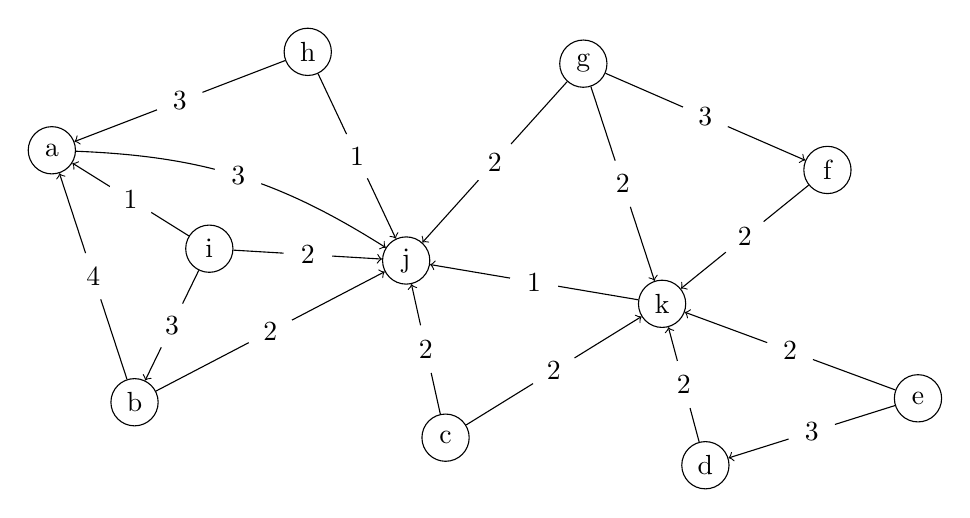
\begin{tikzpicture}
        % Nodes
        \node[circle, draw, minimum size=0.6cm, inner sep=0pt] at (0.5* 0.0, 0.5* 8.5)  (a)    {a};
        \node[circle, draw, minimum size=0.6cm, inner sep=0pt] at (0.5* 2.1, 0.5* 2.1)  (b)    {b};
        \node[circle, draw, minimum size=0.6cm, inner sep=0pt] at (0.5* 10.0, 0.5* 1.2)  (c)    {c};
        \node[circle, draw, minimum size=0.6cm, inner sep=0pt] at (0.5* 16.6, 0.5* 0.5)  (d)    {d};
        \node[circle, draw, minimum size=0.6cm, inner sep=0pt] at (0.5* 22.0, 0.5* 2.2)  (e)    {e};
        \node[circle, draw, minimum size=0.6cm, inner sep=0pt] at (0.5* 19.7, 0.5* 8.0)  (f)    {f};
        \node[circle, draw, minimum size=0.6cm, inner sep=0pt] at (0.5* 13.5, 0.5* 10.7)  (g)    {g};
        \node[circle, draw, minimum size=0.6cm, inner sep=0pt] at (0.5* 6.5, 0.5* 11.0)  (h)    {h};
        \node[circle, draw, minimum size=0.6cm, inner sep=0pt] at (0.5* 4.0, 0.5* 6.0)  (i)    {i};
        \node[circle, draw, minimum size=0.6cm, inner sep=0pt] at (0.5* 9.0, 0.5* 5.7)  (j)    {j};
        \node[circle, draw, minimum size=0.6cm, inner sep=0pt] at (0.5* 15.5, 0.5* 4.6)  (k)    {k};


        \draw[->]  (a) edge[bend left=15] node[circle, fill=white] {3} (j);

        \draw[->]  (b) edge node[circle, fill=white] {4} (a);
        \draw[->]  (b) edge node[circle, fill=white] {2} (j);

        \draw[->]  (c) edge node[circle, fill=white] {2} (j);
        \draw[->]  (c) edge node[circle, fill=white] {2} (k);

        \draw[->]  (d) edge node[circle, fill=white] {2} (k);

        \draw[->]  (e) edge node[circle, fill=white] {3} (d);
        \draw[->]  (e) edge node[circle, fill=white] {2} (k);

        \draw[->]  (f) edge node[circle, fill=white] {2} (k);

        \draw[->]  (g) edge node[circle, fill=white] {3} (f);
        \draw[->]  (g) edge node[circle, fill=white] {2} (j);
        \draw[->]  (g) edge node[circle, fill=white] {2} (k);

        \draw[->]  (h) edge node[circle, fill=white] {3} (a);
        \draw[->]  (h) edge node[circle, fill=white] {1} (j);

        \draw[->]  (i) edge node[circle, fill=white] {1} (a);
        \draw[->]  (i) edge node[circle, fill=white] {3} (b);
        \draw[->]  (i) edge node[circle, fill=white] {2} (j);


        \draw[->]  (k) edge node[circle, fill=white] {1} (j);
    \end{tikzpicture}
    \caption{Upward Graph des Beispielgraphs}
\end{figure}





Aus dieser Definition folgt, dass der kürzeste Pfad zwischen zwei Knoten in $G_u$ ist also mindestens genausolang ist wie in $G$.
% https://cstheory.stackexchange.com/questions/23767/why-is-label-pruning-possible-with-hub-labeling

\todo{Zeiche zwei Suchbäume, jeweils in G und Gu}

\begin{definition}[Downward Graph]
    Sei $G = (V, E)$ und ${vtl} \coloneq V \to \mathbb{N}$ eine \emph{vertex-to-level} Funktion. Dann ist ein upward Graph des Umkehrgraphens $G^T$ ein \emph{downward Graph} zu $G$.
\end{definition}

Ein \emph{Contracted Graph} ist die Datenstruktur, mit deren Hilfe schnell kürzeste Wege gefunden werden können.
Bevor im Folgenden verschiedene Arten beschrieben werden, wie, ein Contracted Graph erstellt werden kann, wird eine allgemeingültige Definition eingeführt.

\begin{algorithm}
    \caption{Construction Hierachies Query}
    \begin{algorithmic}[1]
        \Require Upward-Graph $G_u = (V, E_u)$, Downward-Graph $G_d = (V, E_d)$, Startknoten $s \in V$, Zielknoten $t \in V$
        \Ensure Treffknoten $m \in V \cup \{ {none} \}$, ${dist}_u$, ${pre}_u$, ${dist}_d$, ${pre}_d$
        \State ${dist}_u$, ${pre}_u$ $\leftarrow$ Dijkstra$(G_u, s)$
        \State ${dist}_d$, ${pre}_d$ $\leftarrow$ Dijkstra$(G_d, t)$

        \State
        \State $m \leftarrow {none}$
        \State $d \leftarrow \infty$
        \State

        \ForAll {$v \in V$}
        \If {${dist}_u(v) + {dist}_d(v) < d$}
        \State $m \leftarrow v$
        \State $d \leftarrow {dist}_u(v) + {dist}_d(v)$
        \EndIf
        \EndFor

        \State
        \State \Return $m$, ${dist}_u$, ${pre}_u$, ${dist}_d$, ${pre}_d$
    \end{algorithmic}
\end{algorithm}


Die Suche eines kürzesten Pfades von $u$ nach $v$ auf einem Contracted Graph gestaltet sich nun wie folgt:
Auf $G_u$ wird eine Breitensuche von $u$ und auf $G_d$ eine Breitensuche von $v$ durchgeführt.
\autoref{fig:ch:beispiel_suche} zeigt das auf- und absteigen der Level an einem Beispiel.

Gibt es einen Pfad von $u$ nach $v$, so werden beide Suchen den Knoten $t$ mit dem höchsten Level auf dem kürzesten Pfad finden.
Die kürzeste Pfad Distanz ist dann die Summe der Distanz der upward Suche ($u \to t$) und der downward Suche ($v \to t$).
Der kürzeste Pfad ist der setzt sich aus den beiden Pfaden der upward und downward Suche zusammen, wobei der in beiden Teilen vorkommenden Knoten $t$ in einem Teil entfernt und werden muss.
Da $G_d$ den Pfad von $v$ nach $t$ findet, muss dieser Teil des Pfades invertiert werden, bevor die Teilpfade konkatiniert werden.

\begin{figure}[ht]
    \centering
    \begin{tikzpicture}
        \node[circle, draw] at (0 * 1.5, -5 * 0.75)  (a)    {u};
        \node[circle, draw] at (1 * 1.5, -7 * 0.75)  (b)    {b};
        \node[circle, draw] at (2 * 1.5, -6 * 0.75)  (c)    {c};
        \node[circle, draw] at (3 * 1.5, -1 * 0.75)  (d)    {d};
        \node[circle, draw] at (4 * 1.5, -0 * 0.75)  (e)    {t};
        \node[circle, draw] at (5 * 1.5, -3 * 0.75)  (f)    {f};
        \node[circle, draw] at (6 * 1.5, -2 * 0.75)  (g)    {g};
        \node[circle, draw] at (7 * 1.5, -4 * 0.75)  (h)    {v};

        % draw axis
        \draw[->] (-1, -7 * 0.75) -- (-1, 0) node[above] {Level};

        \draw[->]  (a) -- (d);
        \draw[->]  (d) -- (e);
        \draw[->]  (h) -- (g);
        \draw[->]  (g) -- (e);

        \draw[->, dotted]  (a) -- (b);
        \draw[->, dotted]  (b) -- (c);
        \draw[->, dotted]  (c) -- (d);
        \draw[->, dotted]  (g) -- (f);
        \draw[->, dotted]  (f) -- (e);

    \end{tikzpicture}
    \caption{Beispiel einer Suche in einem Contrated Graph}
    \label{fig:ch:beispiel_suche}
\end{figure}

\begin{beweis}
    Der Beweis der Korrektheit folgt in zwei Schritte.

    \begin{enumerate}
        \item
              Es existiert ein kürzester Pfad von $u$ nach $v$ in $G$ $\Rightarrow$ Er wird in $C$ gefunden.

              Da ${vtl}$ injektiv ist, existiert genau ein Knoten $t$ mit dem höchstem Level. Zerscheide den Pfad $(u, \dotsc, v)$ in zwei Teile:  und $(u, \dotsc, t)$ und $(t, \dotsc, v)$. Die Tupel benachbarten Knoten in $(u, \dotsc, t)$ sind nach \autoref{ch:definition:downward} der Definition des upward Graph Kanten von $G_u$. Daher wird $t$ im upward Graph gefunden. Analog dazu wird $t$ in $G_d$ gefunden, die Tupel benachbarter Knoten im Pfad $(t, \dotsc, v)$ sind nach \autoref{ch:definition:upward} der Definition des downward Graphs Kanten von $G_d$.

              Da die Tupel Kanten der Graphen sind, findet eine Breitensuche sie.

        \item
              Es existiert kein kürzester Pfad von $u$ nach $v$ in $G$ $\Rightarrow$ Es wird in $C$ kein Pfad gefunden gefunden.

              Angenommen, es würde ein Pfad in C gefunden werden. Die Tupel benachbarter Knoten des Pfades müssten dann Kanten in C sein.
              Mindestens einer diese Kanten hätte dann ein Gewicht welches gegen \autoref{ch:definition:legal_edges} der Definition verstoßt.
    \end{enumerate}

    Daher gilt, die Suche der kürzesten Pfad Distanz in $C$ ist äquivalent zu der in $G$
\end{beweis}

\section{Erstellung}

Das Ziel der Contraction Hierarchies ist es aus dem Graph zwei Teilgraphe mit Abkürzungen (\emph{shortcuts}) zu erstellen.
Auf diesen Graphen kann mit einer Breitensuche effizient ein Knoten gefunden werden, der auf dem kürzesten Pfad zwischen zwei Knoten liegt.

\subsection{Contraction}

\begin{definition}[Vertex Contraction]
    Ein Knoten wird wie folgt konktraktiert.

    Für jeden Vorgänger und jeden Nachfolger:
    Wenn der Knoten auf dem einzigen kürzesten Pfad zwischen Vorgänger und Nachfolger liegt, füge einen Shortcut Vorgänger Nachfolger ein.
    Speichere ((Vorgänger, Nachgänger), Knoten) ab.

    Entferne jede Kante zu Vorgänger und Nachfolger.
\end{definition}

Für die verbleibenden Knoten bleibt der kürzeste Pfad erhalten.


\subsubsection{Top-Up}

Wenn $ltv$ gegeben ist, einfach alle Knoten von Level 0 aus startend kontraktieren.
Sammle alle Shortcuts.

Füge alle Shortcuts in den Graphen ein.
Erstelle upward Graph/dopward Graph aus Graph wobei upward  nur Level aufwärts.
downward Graph ist inverser Graph Level downwards.


\todo{überhaupt Möglich weil sum degree**2 zu hoch?}

Für die triangulierten Graphen ist es möglich den klassischen Contraction Hierarchie Algorithmus mit der Knoten-Differenz und Lazy-poping (\cite{geisberger2008contraction}) anzuwenden, wobei auch ein signifikanter Speedup erzielt werden kann. \todo{Tabelle Speedup}
Darauf aufbauend kann auch ein Hub Labeling erstellt werden, wodurch nochmals ein signifikanter Speedup erzielt werden kann.
Für die Sichtbarkeitsgraphen gilt dies jedoch nicht, auf den verwendeten Computern konnte für keinen von ihnen innerhalb von drei Tagen eine Erstellung abgeschlossen werden.
\todo{Wie weit sind sie gekommen? Was ist der größtmögliche Graph, für den dies möglich ist?}
Der Grund hierfür ist naheliegend: Der Algorithmus führt für jeden In-Nachbar eine one-to-many Suche zu allen Out-Nachbarn aus.
Die Durschnitliche Suchtiefe ist dabei sehr hoch, da Knoten des Sichtbarkeitsgraphen mit einer hohen Wahrscheinlichkeit eine Kanten mit großem Gewicht haben, die zum Beispiel über einen Ozean auf die am weitest entfernte Küste zeigt.
Das begrenzen der Suche auf wenige Hops ist dabei auch nicht hilfreich, da die Durschnitliche Hop-Länge von kürzesten Pfaden auf Sichtbarkeitsgraph gering ist eine so begrenzte Suche also viele kürzeste Pfade nicht finden würde.

Daher müssen für die Sichtbarkeitsgraphen andere Methoden gefunden werden.
Die naheliegendste Idee ist das direkte Berechnen der CH Edges und HL Labels.
Dies ist zwar sehr rechenintensiv, es muss für jeden Knoten eine one-to-many bzw. one-to-all Suche durchgeführt werden, dies ist jedoch schneller möglich, also für jeden in-Nachbar eine one-to-many Suche zu berechnen.


\subsubsection{Bottom-Up}

Erstelle $lvt$ Währen dem erstellen.

edge diff.

Greddy lazy poping vs neighbor update.

lazy poping für vis graphen nicht sinvoll?

Neighbor update für vis graphen nicht sinvoll?
Vielleicht nur updaten, nachdem n nachbarn contracted worden?

Vielleicht nur n mal insgesammt updaten? alle 10\% neu berechnen?



Heuristic egde difference (zufall)
Vis graphen haben sehr hohen degree (TODO Beweis).
Daher degree x degree viele checks, das gehtn schnell in die Millionen bis Milliarden.
Idee: betrachte nur ein Subset (tails, heads) und schaue ob und wie genau dieses die Edge difference aproximiert.

Das kann dann wieder für andere Methoden benutzt werden.

Plot hitting set vs bottom-up order


\subsubsection{Ideen}

Verwende eine Heuristik für Contractio


Wir betrachten Vertex v. tail -> v -> head.
Füge shortcut tail -> head ein, wenn tail -> v -> head der einzigste kürzste Weg ist.
Dafür eine one to many without v Vorwärtssuche.
shortcut wenn shortcut cost < dijkstra cost
without kann deutlich teuerer machen (TODO Beweis).

daher besser ohne without. Dann aber shortcut wenn cost <= dijkstra cost.
Die Ungleichung wird also abgeschwächt.
Zusätzlich kann man noch max\_hops anschauen, aber das ist für die Visibility Graphen nur bedingt sinvoll, da kürzste wege nur wenig hops. TODO Beweis

Heuristic.
Statt suche kann man auch heursitc benutzten.
shortcut distance < dijksta cost ==> shortcut distance <= upper bound
also shortcut distance <= upper bound => füge shortcut ein

Used heuristics:
TrivialeHeuristic (all in). Füge jeden shortcut ein.

Landmarks. Gut für größere Entfernungen.
Es reicht zu zeigen, dass shortcut distance > upperbound für ein Landmark ist. Dann bereits kein shortcut.
Viele Landmakrs, weniger shortcuts, mehr checks (vielleicht gibt es Break-Even point?). Wenige Landmarks, mehr shortcuts, weniger checks?
TODO Vielleicht noch check einbauen dass wenn shortcut distance == lower bound, dann shortcut zwingen notwendig ist.
TODO Wenn shortcut distance == lowerbound(head) - lowerbound(tail) dann checken ob tail auf landmark path (head). Oder ist das unnötig nach oben?

CH / HL als Heuristic.
Dann ist lowerbound == upperbound und damit wie dijkstra ohne without. Kann sich unter umständen lohnen.


\section{Hitting Set Berechnung}

\begin{algorithm}
    \caption{Greedy Hitting Set}
    \begin{algorithmic}[1]
        \Require Knotenmenge $V$, Pfade $P$ über $V$
        \Ensure Hitting-Set $H$ als geordnete Menge

        \State $H \gets \emptyset$

        \State

        \While{$P \neq \emptyset$}
        \State Wähle $v \in V$ mit $\abs{ \{ p \mid p \in P \colon v \in p \}}$ maximal.
        \State $H \gets \{v\} \cup H$
        \State $P \gets P \setminus \{p \in P \mid v \in p\}$
        \EndWhile

        \State

        \State \Return $H$
    \end{algorithmic}
\end{algorithm}

Vorraussetzung für das Bruteforcing ist eine Funktion $f \coloneq V \to \mathbb{N}$, welche den Knoten einem \emph{Level}

Level-to-vertex

TODO Edge difference factor
überlegung ist, nur wenige hops. Daher reicht es eigenbtlich direkte Nachbarn anschauen.

Hitting set
Berechne Hitting Set mit Dijkstra oder CH, HL aus vorheriger Runde.
TODO Qualität des Hitting Set durch aproximitation der HL Size.

Bottum up contraction auf graph, verwende dieses für Vis Graph.
TODO

Random


\section{Brute force}

Berechne die Kanten stupide nach Defintion. Hoffnung: Suche ist relativ lokal? TODO Beweis? Avg dijksta rang?

Das mit den Shortcuts ist dann nicht so einfach. TODO Bild


\chapter{Kontraktion in Graphen mit hohen Knotengraden}

Die zuvor beschriebenen klassische Kontraktion stößt bei Graphen mit hohen Knotengraden an ihre Grenzen:
Bei der Kontraktion muss für jeden Vorgängerknoten eine Dijkstra-Suche durchgeführt werden, und für jedes Paar aus Vorgänger- und Nachfolger ist zu prüfen, ob eine Abkürzung eingefügt werden muss.
Um Graphen mit hohen Knotengraden effizent zu kontrakieren ist es daher entscheidend, sowohl die Kontraktion einzelner Knoten als auch die des gesamten Graphen zu beschleunigen.

\section{Kontraktion mit oberer Schranke}
Anstelle einer potenziell rechenintensiven Dijkstra-Suche pro Vorgänger kann eine Heuristik pro Paar aus Vorgänger und Nachfolger eine obere Schranke für den Abstand geben.
Eine Abkürzung wird dann eingefügt, wenn die Länge der potenziellen Abkürzung kleiner oder gleich der oberen Schranke ist.
Damit dies für die Kontraktion eines einzelnen Knotens effizienter ist, muss die Ermittlung der Heuristik für alle Paare eines bestimmten Vorgängers und aller Nachfolger schneller sein als die Dijkstra-Suche.
Damit die Kontraktion des gesamten Graphen effizienter ist, müssen die Folgekosten unnötigerweise eingefügter Kanten kleiner sein als die Summe des Zeitgewinns durch die Verwendung der Heuristik.
Im Follgenden werden verschiedene Heuristiken diskutiert.

\section{Triviale Heurisik}
Die \emph{Triviale Heuristik} setzt die obere Schranke für jedes Knotenpaar auf $\infty$.
Dies bedeutet, dass für jedes Paar aus Vorgänger- und Nachfolgerknoten eine Abkürzung eingefügt wird, unabhängig von der tatsächlichen Distanz zwischen den Knoten.
Unter der Annahme, dass in Graphen mit sehr hohem Knotengrad fast alle Nachbarn bereits mit einer Kante verbunden sind, könnte der Anteil der unnötig eingefügten Abkürzungen im Verhältnis zu den notwendig eingefügten Abkürzungen vernachlässigbar sein.

\section{Vereinfacher Graph}
Sei $G = (V, E)$ der zu Kontraktierende Graph.
Lässt sich zu $G$ effizient ein vereinfachter Graph $G' = (V, E')$ mit $\forall s, t \in V \colon {spd}_{G'} ((s, t)) \geq {spd}_{G} ((s, t))$ konstruieren, so kann dieser zur Berechnung der oberen Schranke verwendet werden, etwa indem die Dijkstra Suchen auf ihm ausgeführt werden.
Alternativ kann $G'$ auch in Contracted oder Hub Graph umgewandelt werden, womit die obere Schranke dann für jedes Vorgänger Nachfolger Paar einzelnen berechnet wird.

Methoden zur Vereinfachung eines Graphens ohne Verkleinerung des Abstandes zweier Knoten werden in dieser Arbeit nicht weiter diskutiert, es ist Anzunehmen, dass die Genauigkeit der oberen Schranke und die Geschwindigkeit der Berechnungen auf dem vereinfachten Graphen im Widerspruch stehen.
Weiter sind solche vereinfachten Graphen im Allgemeinen schwer zu konstruieren.

Jedoch lässt sich diese Methode besonders gut auf die in dieser Arbeit bearbeiteten Sichtbarkeitsgraphen und ihre Triangulierungen anwenden, da zweitere eine obere Schranke für erste liefern und Berechnungen auf Ihnen im Vergleich sehr effizent sind.

\section{Dreickunsgleichung}
Ähnlich zu ALT\cite{goldberg2005computing} kann eine Menge \emph{Hubs} berechnet werden, welche mittels der Dreiecksungleichung eine obere Schranke angeben können.
Ein Hub ist hierbei ein Knoten $l \in V$, für den die Distanz zu und von allen Knoten bekannt ist, die obere Schranke des Abstandes zweier Knoten $s, t \in V$ kann dann durch ${spd}_G ((u, l)) + {spd}((l, u))$ berechnet werden
Liegt $l$ dabei auf einem kürzesten Pfad von $u$ nach $v$, so entspricht der Wert sogar genau dem der kürzesten Pfad Distanz.
Die obere Schranke über mehrere Hubs wird dabei durch die Wahl der kleinsten oberen Schranke bestimmt.
In der Implementation hierfür reicht es sogar, eine obere Schranke zu finden, die kürzer als die potentielle Abkürzung ist, diese kann dann keine otpimale Abkürzung sein.

Die Hubs können dabei über die Berechnung eines Hitting-Sets bestimmt werden.
Durch die Auswahl von Hubs auf die Art steigt Genauigkeit der oberen Schranken mit der Hop-Länge der kürzesten Pfade, da die Wahrscheinlichkeit, dass diese durch einen Hub getroffen wird, steigt.
Durch mehr Hubs steigt allerdings auch der Zeitbedarf der Berechnung der oberen Schranke.

\section{Kombination mehrer oberer Schranken}
Sind für eine Graph mehrere Heuristiken bekannt, so so kann für eine potentielle Abkürzungen aus allen oberen Schranken die kleinste ausgewählt werden.
Dies ist besonders dann sinvoll, wenn die Heuristiken andere Stärken und Schwächen haben.

Insbesondere die Kombination von Dreicksungleichung und vereinfachtem Graph ist hierbei erfeolgsversprechen unter der Annahme, dass die erste für große und zweitere für kleine Hop-Abstände gute obere Schranken liefert.

% TODO das drinnne lassen?
% \section{Datenstrukturen}
% 
% Im Allgemeinen haben wir zwei Anforderungen an die verwendeten Datenstrukturen, welche zur Repräsentation der Graphen verwendet werden: Es muss möglich sein für einen Knoten seine Vorgänger und Nachfolger zu finden und es muss möglich sein Kanten zu verändern oder zu entfernen.
% Diese beiden Ansprüche stehen sich mitunter gegenüber.
% 
% Knoten und Distanzen werde in der Implentierung als uint32 repräsentiert.
% Als Grundbaustein wurden verschiedene Graphen implementiert, welche jeweils nur ihre Nachfolger kennen.
% Damit ein Graph auch seine Vorgänger kennt, wurden jeweils zwei dieser Graphen zusammen benutzt.
% 
% \subsection{VecVecGraph}
% 
% Ein VecVecGraph besteht aus einem Vektor mit jeweils einem Eintrag pro Knoten.
% Dieser Eintrag ist ein Vector über Tuple Knoten $\times$ Distanz, welche nach dem Knoten sortiert sind.
% Der Knoten entspricht dabei dem Kopf einer Kante, ihr Fuß ist der Index in dem ersten Vektor.
% Soll eine Kante gefunden werden, so muss im Vektor, welche mit dem Fuß gefunden wird, eine Binäre Suche nach dem Kopf gemacht werden.
% 
% Das Iterieren über von aus einem Knoten ausgehenden Kanten ist damit effizient, das finden einer bestimmten Kante für kleinere Grade auch.
% Bei größeren Graden kann die Binäre Suche jedoch eine einen negativen Perfomance Overhead darstellen.
% Gleiches gilt für das Einfügen von neuen und Löschen von bestehenden Kanten, denn für größere Grade müssen dafür eine größere Menge an Knoten geschoben werden.
% 
% \subsection{VecHashGraph}
% 
% Ein VecHashGraph besteht wieder aus einem Vektor mit jeweil einem Eintrag pro Knoten, welcher eine HashMap Knoten auf Distanz ist.
% Durch die ausgehenden Kanten kann dann iteriert werden, indem die HashMap, welche zum Fuß gehört aufgerufen wird und durch diese itertiert wird.
% 
% Das Iterieren über diese Kanten ist etwas ineffizienter, da die Einträge in der HashMap nicht konitunierlich im Speicher liegen und dadurch die Cache-Effizent sinkt.
% Dafür wird bei größeren Graden das Finden von spezifischen Kanten, sowie das Einfügen und Löschen effizenter.
% Eine in dieser Arbeit nicht benutzte aber interesannte Datenstruktu ist die HashMap, Effizientes Iterieren und Finden von Kanten mit inefieziennten Einfügen und Löschen verbindet.
% 
% \subsection{VecGraph}
% 
% Soll ein Graph nicht verändert werden, sondern nur zum Finden von Nachbarn in einer Dijkstra Suche benutxt werden, so bietet sich ein VecGraph an.
% Dieser besteht aus zwei Vectoren, einem Index Vektor mit je einem Eintrag pro Knoten der Form Startindex, Stopindex und einem Kanten Vector der Form Knoten, Distanz.
% Aus einem Knoten ausgehende Kanten lassen sich dann finden, indem im Indexvektor der Start- und Stopindex gefunden wird.
% Dieses Paar gibt an, wo im Kantenindex die dazugehörigen Kanten sind.
% Durch die Verwendung des Start- undt Stopindex lassen sich die Kanten von häufig benutzten Knoten an einem Ende des Knotenvektors grupieren, dadurch lässt sich die Wahrscheinlichkeit von Cache-Hits erhöhen.

\chapter{PEOPLE: Predetermined Order, Prunded Label}

Das erstellen von Abkürzungen während der Kontraktion eines Knotes $v$ erfordert mindestens $\abs{\text{Vorgänger}} \cdot \abs{\text{Nachfolger}}$ viele Vergleiche, ob eine Kante einzufügen ist.
Wird zusätzlich noch für jeden Vorgänge eine Dijkstra Suche ausgeführt, so steigt der Zeitbedarf noch einmal deutlich an
Wird eine Warteschlange mit Kanten-Differenz benutzt, so sind alleine für die Initalsierung deren Initialsierung $\sum_{v \in V} \abs{\text{Vorgänger}(v)} \cdot \abs{\text{Nachfolger}(v)}$ Vergleiche notwendig.
Für Graphen, welche Knoten mit einem hohem Grad enthalten, kann dies dazu führen, dass die Kontraktion mancher Knoten nicht mehr in einem sinvollen Zeitrahmen berechenbar ist.
Trotzdem wäre es praktisch, wenn sich die Query-Zeiten von Contraction Hierarchirs und Hierachical Hub Labeling auch auf sie übertragen ließen.

Um die Nachfolgende Definition vorzubereiten, betrachten wir ein Beispiel.
Sei $G = (V, E)$ mit $\supset V \supset \{ u, v, w \}$ und $E = \{ (u, v, {spd}((u, v))), (v, w, {spd}((v, w))) \}$, ein Produkt einer Kontraktion, also zu Beginn mehr Kanten und nicht-isolierte Knoten entiehlt
Es soll nun $v$ kontraktiert werden.
Hierfür wir eine Kante $(u, w, {spd}((u, w)))$ eingefügt und die Kanten $(u, v), (v, w)$ entfernt.
Was bedeuted dies für den enstehenden Contracted Graph $C$?
\begin{enumerate}
    \item
          Alle Knoten, einschließlich $v$ haben ein niedriges Level als $u$ und $w$.
          Inbesondere haben alle Knoten auf allen kürzesten Pfaden von $u$ nach $w$, also die, die bereits kontraktiert wurden, ein niedrigeres Level.

    \item
          $(u, w) \in E_u$ gilt genau dann, wenn $w$ das größte Level auf allen Pfaden von $u$ nach $w$.
          $(w, u) \in E_d$ gilt, wenn $u$ das größte Level hat.
\end{enumerate}

Es kann nun gezeigt werden, dass auch die Rückrichtung gilt, also dass basienden auf dieser Chracterisierung ein Contracted Graph gebildet werden kann.

% \begin{definition}[max-on-paths]
%     Sei $G = (V, E)$ und ${vtl}$ eine \emph{vertex-to-level} Funktion dazu.
%     Dann ist die \emph{max-on-paths} Funktion ${mop} \colon V \times V \to L$ definiert als größte Level eines Knotens auf allen kürzesten Pfaden zwischen zwei Knoten.
% \end{definition}

\begin{definition}[Upward Graph]\label{people:def:upward_graph}
    Sei $G = (V, E)$ und ${vtl}$ eine \emph{vertex-to-level} Funktion dazu. Dann ist $G_u = (V, E_u)$ ein \emph{upward Graph} zu $G$ wenn gilt:

    Für jeden Knoten $t \in V$ ist $(t, h, {spd}((t, h))) \in E_u$ mit $h \in V$ wenn $h$ das größte und $t$ das zweitgrößte Level auf allen kürzesten Wege auf $G$ von $t$ nach $h$ hat.
\end{definition}

Betrachten wir das ganze an dem bereits definierten Beispielgraph.
Sei ${vtl}$ definiert durch die Abbildung in \autoref{ch::fig::vtl_abbildung} definiert.
Durch Anwendung der Definition \ref{people:def:upward_graph} ergibt sich der in \autoref{ch::fig::upward_graph} gezeigte Upward Graph.

\begin{table}[ht]
    \centering
    \begin{tabular}{lllllllllllll}
        Vertex & a & b & c & d & e & f & g & h & i & j  & k & \\
        Level  & 8 & 7 & 3 & 6 & 2 & 5 & 1 & 4 & 0 & 10 & 9 &
    \end{tabular}
    \caption{${vtl}$ Beispielfunktion}
    \label{ch::fig::vtl_abbildung}
\end{table}


\begin{figure}[ht]
    \centering
    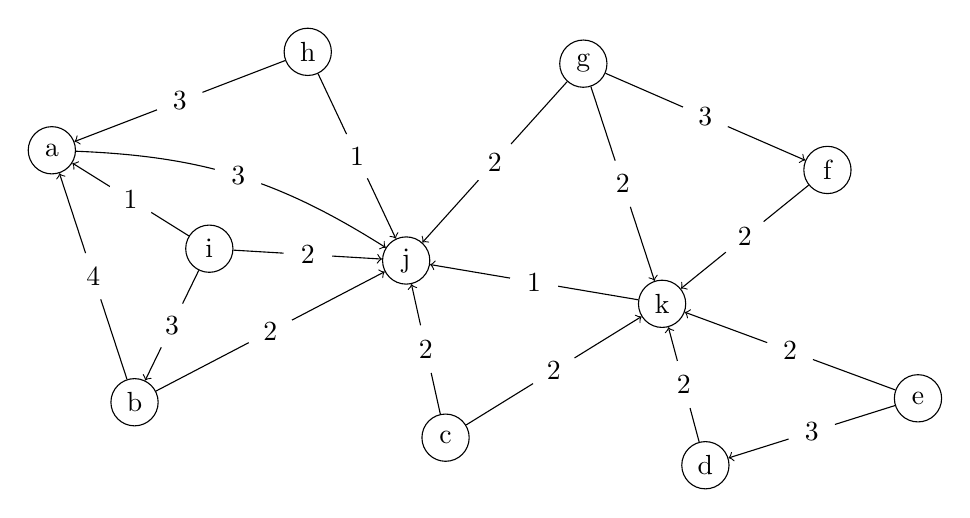
\begin{tikzpicture}
        % Nodes
        \node[circle, draw, minimum size=0.6cm, inner sep=0pt] at (0.5* 0.0, 0.5* 8.5)  (a)    {a};
        \node[circle, draw, minimum size=0.6cm, inner sep=0pt] at (0.5* 2.1, 0.5* 2.1)  (b)    {b};
        \node[circle, draw, minimum size=0.6cm, inner sep=0pt] at (0.5* 10.0, 0.5* 1.2)  (c)    {c};
        \node[circle, draw, minimum size=0.6cm, inner sep=0pt] at (0.5* 16.6, 0.5* 0.5)  (d)    {d};
        \node[circle, draw, minimum size=0.6cm, inner sep=0pt] at (0.5* 22.0, 0.5* 2.2)  (e)    {e};
        \node[circle, draw, minimum size=0.6cm, inner sep=0pt] at (0.5* 19.7, 0.5* 8.0)  (f)    {f};
        \node[circle, draw, minimum size=0.6cm, inner sep=0pt] at (0.5* 13.5, 0.5* 10.7)  (g)    {g};
        \node[circle, draw, minimum size=0.6cm, inner sep=0pt] at (0.5* 6.5, 0.5* 11.0)  (h)    {h};
        \node[circle, draw, minimum size=0.6cm, inner sep=0pt] at (0.5* 4.0, 0.5* 6.0)  (i)    {i};
        \node[circle, draw, minimum size=0.6cm, inner sep=0pt] at (0.5* 9.0, 0.5* 5.7)  (j)    {j};
        \node[circle, draw, minimum size=0.6cm, inner sep=0pt] at (0.5* 15.5, 0.5* 4.6)  (k)    {k};


        \draw[->]  (a) edge[bend left=15] node[circle, fill=white] {3} (j);

        \draw[->]  (b) edge node[circle, fill=white] {4} (a);
        \draw[->]  (b) edge node[circle, fill=white] {2} (j);

        \draw[->]  (c) edge node[circle, fill=white] {2} (j);
        \draw[->]  (c) edge node[circle, fill=white] {2} (k);

        \draw[->]  (d) edge node[circle, fill=white] {2} (k);

        \draw[->]  (e) edge node[circle, fill=white] {3} (d);
        \draw[->]  (e) edge node[circle, fill=white] {2} (k);

        \draw[->]  (f) edge node[circle, fill=white] {2} (k);

        \draw[->]  (g) edge node[circle, fill=white] {3} (f);
        \draw[->]  (g) edge node[circle, fill=white] {2} (j);
        \draw[->]  (g) edge node[circle, fill=white] {2} (k);

        \draw[->]  (h) edge node[circle, fill=white] {3} (a);
        \draw[->]  (h) edge node[circle, fill=white] {1} (j);

        \draw[->]  (i) edge node[circle, fill=white] {1} (a);
        \draw[->]  (i) edge node[circle, fill=white] {3} (b);
        \draw[->]  (i) edge node[circle, fill=white] {2} (j);


        \draw[->]  (k) edge node[circle, fill=white] {1} (j);
    \end{tikzpicture}
    \caption{Upward Graph des Beispielgraphs}
    \label{ch::fig::upward_graph}
\end{figure}

Die Definition des Downward Graphens erfolgt nun analog zu der des Upward Graphens:

\begin{definition}[Downward Graph]
    Sei $G = (V, E)$ und ${vtl} \coloneq V \to \mathbb{N}$ eine \emph{vertex-to-level} Funktion. Dann ist ein upward Graph des Umkehrgraphens $G^T$ ein \emph{downward Graph} zu $G$.
\end{definition}

Wenn ein Graph ungerichtet ist, dann ist er äuivalent zu seinem Umkehrgraphen und dann ist auch der Upward und Downward Graph äuivalent.
Daher entspricht \autoref{ch::fig::upward_graph} gleichzeitig auch dem Downward Graph des Beispielgraphens.



\chapter{Ergebnisse}




Für jeden der Graphen wurde mittels

Hitting Set Berechnung.


Wieviel Elemente das Hitting Set reichen aus um x \% aller Pfade zu treffen?


Es war mir möglich CH und HL zu brute forcen.

Tabelle Speedup, CH average edge degree, HL average label size

Mit CH, HL konnte ich bessere Hitting sets berechnen und damit noch bessere CH und HL  berechnen



Ich konnte auf den triangulierten Graphen mit Alt eine CH berechnen.



Das Merging war erstaunlich langsam. Das ist weil sehr viele Labels gemerged werden müssen.


TODO kann ich mit trianguliertem HL und Vertex Order Sichtbarkeitsgraph CH berechnen?
Vielleicht noch ALT? ALT für große Entfernungen, tria HL für kurze?


\printbibliography

\end{document}